\documentclass[14pt,a4paper]{extarticle}
\usepackage[T2A]{fontenc}
\usepackage[utf8]{inputenc}
\usepackage[english,russian]{babel}
\usepackage{lmodern}
\usepackage{geometry}
\usepackage{array}
\usepackage{tabularx}
\usepackage{longtable}
\usepackage{ltablex}
\usepackage{booktabs}
\usepackage{hyperref}
\usepackage{indentfirst}
\usepackage{microtype}
\usepackage{graphicx}
\usepackage{setspace}
\usepackage{listings}
\usepackage{graphicx}
\usepackage{caption}
\usepackage{float}
\usepackage{tocloft}
\usepackage{titlesec}
\usepackage{newtxtext,newtxmath}

\titleformat{\section}        % форматируем \section
  {\normalfont\bfseries}      % стиль: обычный + жирный
  {\thesection.}              % номер секции с точкой
  {2mm}                       % расстояние между номером и текстом
  {}                           % перед заголовком можно добавить что-то
\titlespacing*{\section}{1.5cm}{*3}{*1}  % {отступ слева}{отступ сверху}{отступ снизу}

\captionsetup{justification=centering}
\renewcommand{\ttdefault}{cmtt}
\keepXColumns
\setlength{\parindent}{3em}
\newgeometry{left=2.5cm,right=2.5cm,top=3cm,bottom=2.5cm}

\renewcommand{\contentsname}{\hspace*{4em}{\smallСодержание}}
\setlength{\cftbeforesecskip}{0.5em}
\renewcommand{\cftsecleader}{\cftdotfill{\cftdotsep}}
\renewcommand{\cftsecaftersnum}{.\hspace{2mm}}

\title{Отчёт по "Программно-аппаратные средства интеллектуальных систем"}
\author{Выполнил студент группы М-РИТ-25-1, Станиславчук Сергей}

\begin{document}

\setstretch{1.5}
\noindent
\begin{minipage}[t]{0.01\textwidth}
    \includegraphics{~/programmer/++Programmer/5_1/LSTU.jpg}
\end{minipage}%
\begin{minipage}[c]{1.1\linewidth}
    \centering
    {\small
    МИНИСТЕРСТВО НАУКИ И ВЫСШЕГО ОБРАЗОВАНИЯ РФ \\[1em]
    ФЕДЕРАЛЬНОЕ ГОСУДАРСТВЕННОЕ БЮДЖЕТНОЕ \\
    ОБРАЗОВАТЕЛЬНОЕ УЧРЕЖДЕНИЕ ВЫСШЕГО ОБРАЗОВАНИЯ \\
    «ЛИПЕЦКИЙ ГОСУДАРСТВЕННЫЙ ТЕХНИЧЕСКИЙ УНИВЕРСИТЕТ»
    }
\end{minipage}%

\vspace{3em}

\noindent
\hspace{1em}%
\begin{minipage}[t]{0.8\textwidth}
\textbf{Институт} \hspace{2em} компьютерных наук \\
\textbf{Кафедра} \hspace{2em} автоматизированных систем управления
\end{minipage}


\vspace{6em}

\begin{center}
\textbf{ПРАКТИЧЕСКАЯ РАБОТА №4} \\
по дисциплине \\ <<Программно-аппаратные средства интеллектуальных систем>>
\end{center}

\vspace{6em}

\noindent
\begin{tabular*}{\textwidth}{@{\extracolsep{\fill}} l c r }
    Студент М-РИТ-25-1 & \makebox[4cm]{\hrulefill} & Станиславчук С.М. \\[2em]
Руководитель & \\
Ст. преподаватель & \makebox[4cm]{\hrulefill} & Болдырихин О.В. \\
\end{tabular*}

\vfill
\begin{center}
    Липецк, 2025
\end{center}

\thispagestyle{empty}

\newpage
\tableofcontents
\newpage

\section{Задание, конкретизированное вариантом}
\begin{sloppypar}
Цель работы - исследование взаимозависимости между архитектурными
    характеристиками суперкомпьютерных систем рейтинга TOP500 и их
    текхнико-эксплуатационными показателями.

    Задание 1. Сгруппировать системы одного списка по заданному архитек-
    турному признаку (характеристике):
    1. Архитектура CPU: Intel Xeon, AMD EPYC, Fujitsu A64FX, IBM POWER, NVIDIA GRACE.
    2. Гетерогенность: с ускорителями и без ускорителей.
    3. Ускоритель: NVIDIA (A100, H100, P100, V100, H200 и др.), AMD Instinct, Intel Xeon Phi.
    4. Архитектура суперкомпьютера: Cluster, MPP.
    5. Интерконнект: Ethernet, InfiniBand, Omni-Path, Slingshot.
    Они соответствуют номерам строк в таблице 4.1.

    Построить диаграмму размаха (box plot) или скрипичную диаграмму (violin
    plot) для заданного показателя по каждой группе. Сравнить группы по
    распределению значений показателя, среднему значению показателя, разбросу
    значений показателя. Показатели те же, что и в практической работе №3 (см.
    табл. 3.1), они соответствуют номерам столбцов в таблице 4.1

    Номер рейтинга для показателей 1, 2, 4, 5, 7, 9-13 выбирается по формуле:
    \[
        V = N - L + 1,
    \]
\end{sloppypar}

    где $N$ - номер текущего (последнего рейтинга),
        \newline\indent
        $L$ - номер студента в списке.

    Вариант по таблице: 17. \newline\indent
    Номер строки 3 (Графический ускоритель), номер столбца 1 (Rpeak).
    \[
        V = 66 - 17 + 1 = 50
    \]

    Этот номер соответствует рейтингу 2017.11 (см. приложение 1)
\newpage
\section{Описание исследуемых характеристик и показателей}

\begin{sloppypar}
Rpeak - теоретический максимум производительности. Определяется путем умножения
количества единиц измерения с плавающей запятой на процессор, умноженное на
количество команд с плавающей запятой, которые могут быть выполнены в секунду.
Измеряется в GFLOPS

Графический процессор (ускоритель) (GPU) - это специализированная электронная
схема, предназначенная для цифровой обработки изображений и ускорения
компьютерной графики, которая присутствует либо в качестве компонента на
дискретной видеокарте, либо встроена в материнские платы, мобильные телефоны,
персональные компьютеры, рабочие станции и игровые консоли. Графические
процессоры все чаще используются для обработки искусственного интеллекта
благодаря ускорению линейной алгеброй, которое также широко используется в
графической обработке.

Хотя единого определения этого термина не существует и он может быть
использован для описания любой системы отображения видео, в современном
использовании графический процессор включает в себя возможность внутреннего
выполнения вычислений, необходимых для различных графических задач, таких как
поворот и масштабирование 3D-изображений, и часто дополнительную возможность
запуска пользовательских программ, известных как шейдеры. Это контрастирует с
более ранними графическими контроллерами, известными как контроллеры
видеодисплея, которые не имели внутренних вычислительных возможностей, или
блиттерами, которые выполняли только базовые операции перемещения в памяти.
Современные графические процессоры появились в 1990-х годах, добавив
возможность выполнять такие операции, как рисование линий и текста, без помощи
процессора, а позже добавили функциональность 3D.

Графические функции, как правило, независимы, и это позволяет реализовывать эти
задачи на отдельных вычислительных машинах. Современные графические процессоры
содержат сотни или тысячи вычислительных блоков. Это сделало их полезными для
неграфических вычислений, связанных с затруднительно параллельными задачами,
из-за их параллельной структуры. Способность графических процессоров быстро
выполнять огромное количество вычислений привела к их внедрению в различных
областях, включая искусственный интеллект (ИИ), где они превосходно справляются
с задачами, требующими большого объема данных и вычислений. Другие
неграфические приложения включают в себя обучение нейронных сетей и майнинг
криптовалют.

\end{sloppypar}

\section{Исходные данные}

В качестве исходных данных используются результаты
рейтинга TOP500 ноября 2017 года.

\section{Использованные программные средства}
Для выполнения анализа использовался язык программирования Python 3.
Необходимые библиотеки устанавливались с помощью команды:

\begin{sloppypar}
\texttt {pip install re lxml mapplotlib pandas numpy requests tabulate}
\end{sloppypar}

С помощью библиотеки \texttt{requests} выполнялось автоматическое скачивание XML-файлов с сайта \texttt{top500.org}

Модуль «\texttt{lxml.etree}» применялся для разбора структуры XML. Из каждого
документа (рейтинга) извлекается значение <<\texttt{top500:computer}>> с
помощью функции \texttt{findtext}, затем в каждой извлечённой строке ищется 3
группы графических ускорителей: <<\texttt{NVIDIA|A100|H100|P100|V100|H200}>>
или <<\texttt{AMD|INSTINCT}>> или <<\texttt{INTEL|XEON PHI}>> (без учета
регистра) с помощью функции \texttt{search}.
Для поиска Rpeak, извлекается значение <<\texttt{top500:r-peak}>> конвертируется в тип float.
Найденные данные добавляются в массив пар \texttt{ accelerator : rpeak } для последующей обработки.

Результаты записываются в единую таблицу (DataFrame) с помощью библиотеки
\texttt{pandas} и сохраняются в файл \texttt{top500\_efficiency.csv}.
Исходя из полученной таблицы, строится boxplot, в котором: ,
\newlineПо горизонтали - значения Rpeak.
\newlineПо вертикали - производитель GPU.

Текст программы представлен в приложении 2.

\newpage
\section{Группировка систем по заданному признаку. Построение диаграмм.}
    Полученная таблица соответствий "Производитель Ускорителя":"Rpeak"
    для 50 рейтинга TOP500 2017.11 (первые 10 строк), представлена на рисунке 1.

\begin{figure}[H]
    \label{fig:table}
    \centering
    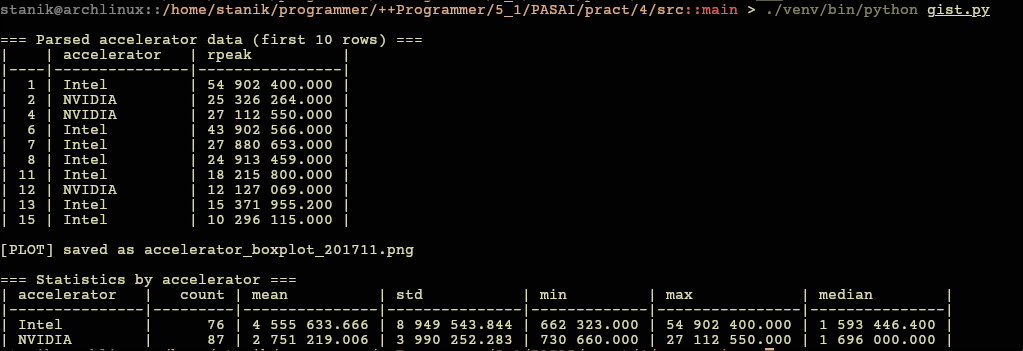
\includegraphics[width=0.78\textwidth]{pic1.png}
    \refstepcounter{figure}
    \caption*{Рисунок \thefigure\ — Таблица "Ускоритель - Rpeak" среди суперкомпьютеров (2017.11)}
\end{figure}

    Boxplot без ограничений позволит увидеть значения, которые сильно отбились от нормы
    - они отмечены полыми кружочками. Хоть и сами ящики с усами трудно
    рассматриваемы на этой картинке, ввиду выличины значения Rpeak у самых
    теоретически мощных суперкомпьютеров. Boxplot полученной таблицы
    представлен на рисунке 2.

\begin{figure}[H]
    \label{fig:histogram}
    \centering
    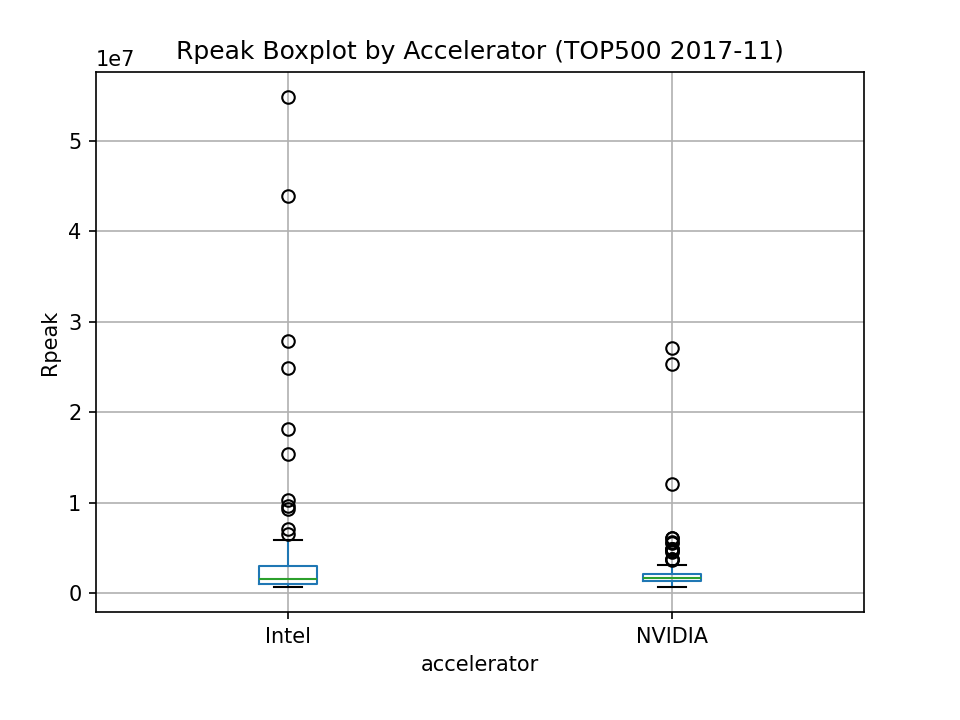
\includegraphics[width=0.9\textwidth]{pic2.png}
    \refstepcounter{figure}
    \caption*{Рисунок \thefigure\ — Ящики с усами (без ограничений по Rpeak))}
\end{figure}

    Boxplot с ограничением по показателю Rpeak позволит увидеть те самые ящики
    с усами, которые и представляют большинство суперкомпьютеров. Boxplot
    полученной таблицы с ограничением по Rpeak представлен на рисунке 3.

\begin{figure}[H]
    \label{fig:histogram}
    \centering
    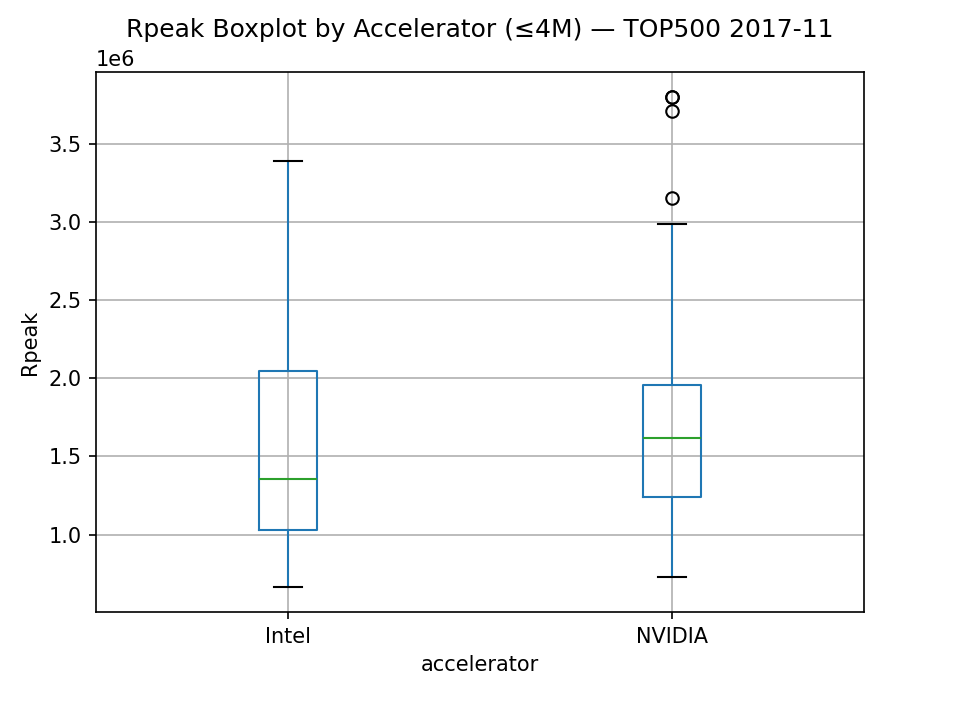
\includegraphics[width=0.9\textwidth]{pic3.png}
    \refstepcounter{figure}
    \caption*{Рисунок \thefigure\ — Ящики с усами (ограничение по $Rpeak <= 4\,000\,000$))}
\end{figure}
\section{Результат сравнения групп}
Среди представленных групп нет AMD Instinct, т.к. эта технология впервые появилась
лишь в рейтинге TOP500 2020 г.

График показывает, что у Intel встречаются отдельные конфигурации с крайне
высоким Rpeak — десятки миллионов и выше. Эти значения лежат значительно выше
верхнего уса, то есть представляют собой чистые выбросы. Они отражают
присутствие крупных систем, использующих масштабируемые многоузловые
процессорные решения.

При этом основная масса систем с Intel-ускорением лежит ближе к низам
диапазона. Ящик у Intel расположен в области порядка 1.5 млн. Rpeak, с медианой в 1.4 млн,
что означает, что большинство систем демонстрируют умеренную производительность на
узел и лишь единичные установки выводят Intel на экстремумы.

Картина у NVIDIA похожа, но выбросы распределены иначе. У NVIDIA тоже есть
системы с Rpeak, уходящими далеко за пределы нормального диапазона, однако эти
выбросы выглядят менее радикальными по сравнению с интеловскими пиками в полном
графике. Ящик NVIDIA расположен примерно на тех же уровнях, что и интеловский,
но медиана у NVIDIA чуть выше (1.6 м), что говорит о том, что среднестатистическая
система с NVIDIA-ускорителем выдает более высокое значение Rpeak, чем
большинство систем Intel.

Intel показывает огромный размах значений, с отдельными системами-гигантами,
которые становятся мощнейшими выбросами. NVIDIA же формирует более высокую
медиану в «рабочем» диапазоне и меньшую вариативность, что говорит о более
стабильном и предсказуемом ускорении на GPU.

Таким образом, Intel на конец 2017 года доминировала в верхних экстремумах, но NVIDIA
выглядила сильнее в массовом среднем сегменте — типичная система с GPU имеет
более высокую пиковой производительность, чем типичная система на основе
Intel-ускорителей.

\section{Задание 2. Упорядочивание списка по заданному показателю. Анализ архитектурных характеристик компьютеров верхней и нижней части списка}

    Полученная таблица агрегированных значений
    для 50 рейтинга TOP500 2017.11, представлена на рисунке 4.

\begin{figure}[H]
    \label{fig:histogram}
    \centering
    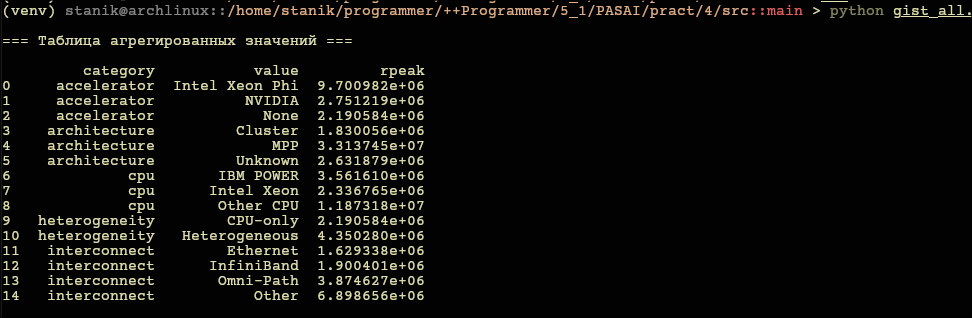
\includegraphics[width=0.9\textwidth]{pic4.png}
    \refstepcounter{figure}
    \caption*{Рисунок \thefigure\ — Таблица агрегированных значений}
\end{figure}

    Полученная категориальная тепловая карта (heatmap) средних значений Rpeak,
    где:
    \newline\indentось X - архитекрутрные характеристики,
    \newline\indentось Y - конкретные категории,
    \newline\indentцвет - средний Rpeak для группы

    представлена на рисунке 5.

\begin{figure}[H]
    \label{fig:histogram}
    \centering
    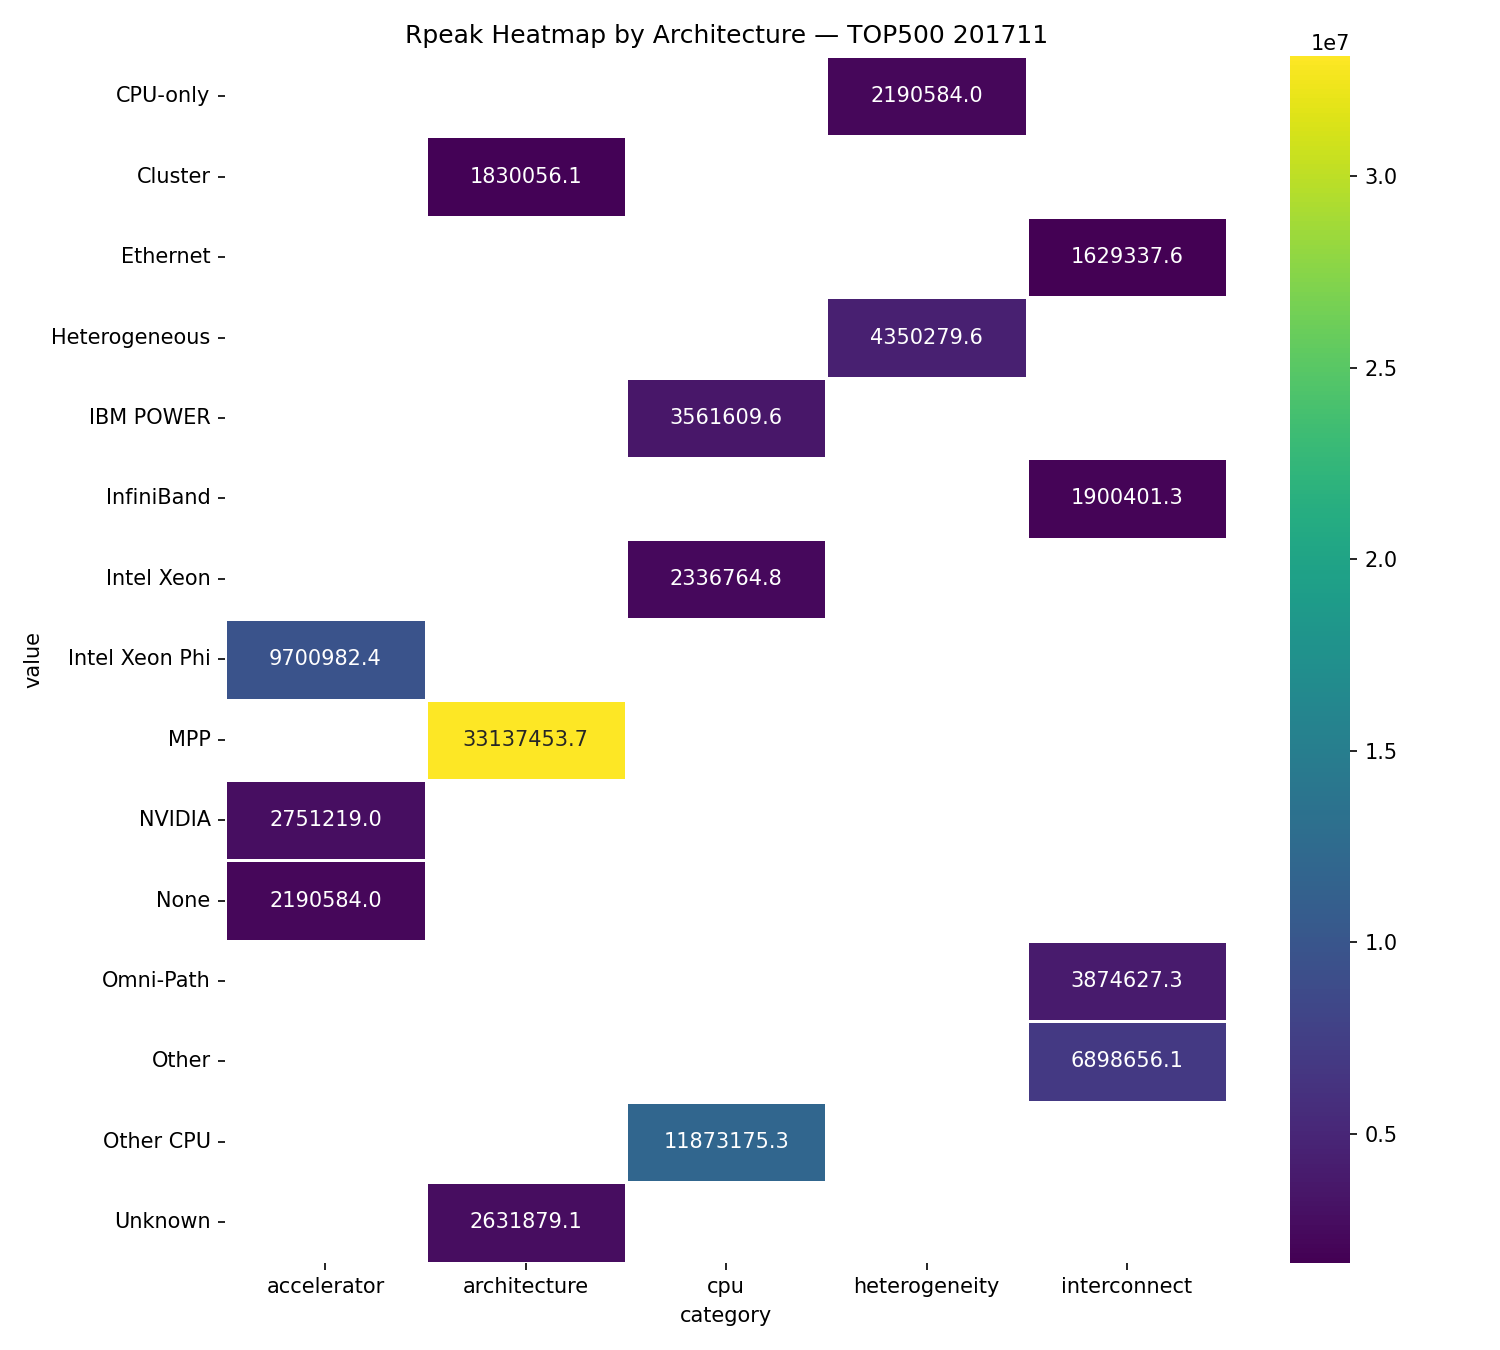
\includegraphics[width=0.9\textwidth]{pic5.png}
    \refstepcounter{figure}
    \caption*{Рисунок \thefigure\ — Категориальная тепловая карта средних значений Rpeak}
\end{figure}

Высокие Rpeak.
1) MPP-архитектуры (Massively Parallel Processing)
$ Rpeak = 3.3*10^7 $
Самая высокая цифра на карте. Системы, созданные как единые аппараты с глубокой внутреннея связности
стабильно дают макс. производительность.

2) Intel Xeon Phi
$ Rpeak = 9.7*10^6 $
Старые MIC-ускорители Intel показывают второе место. Вывод: в эпоху 2010–2020
серьёзную производительность давали многоядерные сопроцессоры Xeon Phi. Они
вытягивали топовые показатели благодаря большому числу ядер.

3) Интерконнекты Omni-Path и InfiniBand

$ Omni-Path = 3.87*10^6 $

$
InfiniBand = 1.9*10^6
$

Omni-Path выглядит сильнее — не удивительно: он проектировался под HPC как
более дешёвая альтернатива InfiniBand, но в мощных суперкомпьютерах его
использовали реже. Быстрый кластерный интерконнект — критичен для верхушки рейтинга.

4) Heterogeneous (гетерогенные системы)

$
Rpeak = 4.35*10^6
$

Гетерогенность даёт хороший прирост. Это <<CPU + GPU>> или <<CPU + ускоритель>>.

Именно смешанные конфигурации дают высокие показатели.

5) NVIDIA GPU как ускорители

$
Rpeak = 2.75*10^6
$

Да, ниже Intel Phi, но выше CPU-only.

Низкие Rpeak.

1) CPU-only системы

$
Rpeak = 2.19*10^6
$

Очевидно: без ускорителей потолок производительности ниже в разы.

2) Ethernet-интерконнект

$
Rpeak = 1.62*10^6
$

Обычный Ethernet не годится для HPC-масштаба.
Он и есть маркер низового сегмента рейтинга.

3) Архитектура Cluster

$
Rpeak = 1.83*10^6
$

Классические кластеры без специализированных ускорителей/высокоскоростных сетей остаются на нижних позициях.

4) Неизвестные / прочие

$
Unknown = 2.63*10^6
$

$
Other CPU = 1.18*10^6
$

$Other = 6.89*10^6$ (аномалия, вероятно единичный мощный экземпляр)

По сути — такие отметки говорят о меньшей системности и о единичных машинах вне основных стандартов.

\section{Выводы по результатам исследования}
В ходе исследования был выполнен разбор данных рейтинга TOP500, включающий
парсинг XML-файлов, агрегацию показателей производительности (Rpeak и Rmax) и
отнесение суперкомпьютеров к группам по ключевым архитектурным характеристикам:
тип процессоров, гетерогенность, наличие ускорителей, тип архитектуры (кластер
или MPP) и применяемый интерконнект. На основе этих данных построена тепловая
карта среднего Rpeak по каждой категории, что позволило выявить общие
закономерности, характерные для верхней и нижней части рейтинга.

Во-первых, лидирующие по производительности системы обладают чётко выраженными
архитектурными особенностями. Максимальные показатели Rpeak принадлежат машинам
класса MPP (Massively Parallel Processing), представляющим собой монолитные
высоко специализированные суперкомпьютеры с глубокой внутренней
параллельностью. Существенный вклад в высокую производительность дают
гетерогенные системы, использующие сочетание CPU и ускорителей (GPU). Особенно
заметны результаты конфигураций с NVIDIA GPU, а также устаревших, но всё ещё
мощных ускорителей Intel Xeon Phi. Важную роль играет и высокоскоростной
интерконнект: системы с Omni-Path и InfiniBand стабильно показывают значительно
более высокие Rpeak, чем кластеры на базе обычного Ethernet. Это подтверждает,
что верхняя часть рейтинга формируется за счёт архитектур, максимизирующих
параллелизм и пропускную способность межузловых соединений.

Во-вторых, нижние позиции рейтинга занимают системы с простыми и недорогими
архитектурами. Кластеры «CPU-only», построенные без ускорителей, демонстрируют
заметно более низкую пиковую производительность. В этой же группе находятся
системы, использующие стандартный Ethernet как интерконнект, что существенно
ограничивает масштабируемость и снижает эффективность распределённых
вычислений. Классические кластерные архитектуры без специализированных сетевых
решений или ускорителей закономерно располагаются внизу рейтинга, поскольку не
способны обеспечить необходимую плотность вычислений и пропускную способность
обмена данными.

Таким образом, исследование подтверждает устойчивый тренд HPC-индустрии: рост
производительности в суперкомпьютерах достигается не за счёт увеличения частот
или количества CPU, а через глубоко параллельные, гетерогенные и
высокоскоростные архитектуры. В верхней части рейтинга доминируют системы,
использующие ускорители и специализированные интерконнекты, тогда как нижняя
часть представлена традиционными кластерными решениями с ограниченными
коммуникационными возможностями. Эти результаты согласуются с мировой практикой
проектирования суперкомпьютеров последних лет и отражают общий переход HPC к
гетерогенным системам и сетям с высокой пропускной способностью.

\newpage
\section*{Приложение 1. Номера всех рейтингов TOP500}
\begin{verbatim}

     1	TOP500_199306.xml
     2	TOP500_199311.xml
     3	TOP500_199406.xml
     4	TOP500_199411.xml
     5	TOP500_199506.xml
     6	TOP500_199511.xml
     7	TOP500_199606.xml
     8	TOP500_199611.xml
     9	TOP500_199706.xml
    10	TOP500_199711.xml
    11	TOP500_199806.xml
    12	TOP500_199811.xml
    13	TOP500_199906.xml
    14	TOP500_199911.xml
    15	TOP500_200006.xml
    16	TOP500_200011.xml
    17	TOP500_200106.xml
    18	TOP500_200111.xml
    19	TOP500_200206.xml
    20	TOP500_200211.xml
    21	TOP500_200306.xml
    22	TOP500_200311.xml
    23	TOP500_200406.xml
    24	TOP500_200411.xml
    25	TOP500_200506.xml
    26	TOP500_200511.xml
    27	TOP500_200606.xml
    28	TOP500_200611.xml
    29	TOP500_200706.xml
    30	TOP500_200711.xml
    31	TOP500_200806.xml
    32	TOP500_200811.xml
    33	TOP500_200906.xml
    34	TOP500_200911.xml
    35	TOP500_201006.xml
    36	TOP500_201011.xml
    37	TOP500_201106.xml
    38	TOP500_201111.xml
    39	TOP500_201206.xml
    40	TOP500_201211.xml
    41	TOP500_201306.xml
    42	TOP500_201311.xml
    43	TOP500_201406.xml
    44	TOP500_201411.xml
    45	TOP500_201506.xml
    46	TOP500_201511.xml
    47	TOP500_201606.xml
    48	TOP500_201611.xml
    49	TOP500_201706.xml
    50	TOP500_201711.xml
    51	TOP500_201806.xml
    52	TOP500_201811.xml
    53	TOP500_201906.xml
    54	TOP500_201911.xml
    55	TOP500_202006.xml
    56	TOP500_202011.xml
    57	TOP500_202106.xml
    58	TOP500_202111.xml
    59	TOP500_202206.xml
    60	TOP500_202211.xml
    61	TOP500_202306.xml
    62	TOP500_202311.xml
    63	TOP500_202406.xml
    64	TOP500_202411.xml
    65	TOP500_202506.xml
    66	TOP500_202511.xml

\end{verbatim}

\newpage
\section*{Приложение 2. Код программы 1}

\begin{verbatim}

#!/usr/bin/env python3

import os
import re
import pandas as pd
import matplotlib.pyplot as plt
from lxml import etree
from tabulate import tabulate

XML_DIR = "xml"
XML_FILE = "TOP500_201711.xml"

OUT_PLOT = "accelerator_boxplot_201711.png"


def load_xml(fname):
    path = os.path.join(XML_DIR, fname)
    if not os.path.exists(path):
        print(f"[ERR] missing XML file: {path}")
        return None
    with open(path, "rb") as f:
        return etree.fromstring(f.read())


def classify_accelerator(text):
    if not text:
        return "Other"
    t = text.upper()

    if re.search(r"NVIDIA|A100|H100|P100|V100|H200", t):
        return "NVIDIA"

    if "AMD" in t or "INSTINCT" in t:
        return "AMD"

    if "XEON PHI" in t or "INTEL" in t:
        return "Intel"

    return "Other"


def parse_list(root):
    ns = {"top500": root.nsmap.get("top500")}

    rows = []

    for site in root.findall("top500:site", namespaces=ns):
        computer = site.findtext("top500:computer", default="", namespaces=ns)
        rpeak = site.findtext("top500:r-peak", default="", namespaces=ns)

        try:
            rpeak_val = float(rpeak)
        except:
            continue

        accel = classify_accelerator(computer)

        rows.append({
            "accelerator": accel,
            "rpeak": rpeak_val
        })

    return rows


# === форматирование чисел ===
def fmt(x):
    try:
        return f"{x:,.3f}".replace(",", " ")
    except:
        return x


def main():
    root = load_xml(XML_FILE)
    if root is None:
        return

    rows = parse_list(root)
    df = pd.DataFrame(rows)

    # оставляем только три основные группы
    df = df[df["accelerator"].isin(["NVIDIA", "AMD", "Intel"])]

    print("\n=== Parsed accelerator data (first 10 rows) ===")
    print(tabulate(df.head(10).map(fmt), headers="keys", tablefmt="github"))

    # === boxplot ===
    plt.figure(figsize=(10, 6))
    df.boxplot(column="rpeak", by="accelerator")
    plt.title("Rpeak Boxplot by Accelerator (TOP500 2017-11)")
    plt.suptitle("")
    plt.ylabel("Rpeak")
    plt.savefig(OUT_PLOT, dpi=150)
    plt.close()

    print(f"\n[PLOT] saved as {OUT_PLOT}")

    # === stats ===
    stats = df.groupby("accelerator")["rpeak"].agg(
        ["count", "mean", "std", "min", "max", "median"]
    )

    print("\n=== Statistics by accelerator ===")
    print(tabulate(stats.map(fmt), headers="keys", tablefmt="github"))


if __name__ == "__main__":
    main()
\end{verbatim}

\newpage
\section*{Приложение 3. Код программы 2}

\begin{verbatim}

#!/usr/bin/env python3
import os
import pandas as pd
import matplotlib.pyplot as plt
import seaborn as sns
from lxml import etree

XML_DIR = "xml"
TARGET = "201711"      # рейтинг
AGG = "mean"           # можно median


# === Классификаторы ===

def detect_cpu(text):
    txt = text.lower()
    if "xeon" in txt:
        return "Intel Xeon"
    if "epyc" in txt:
        return "AMD EPYC"
    if "a64fx" in txt:
        return "Fujitsu A64FX"
    if "power" in txt:
        return "IBM POWER"
    if "grace" in txt:
        return "NVIDIA GRACE"
    return "Other CPU"


def detect_accel(text):
    txt = text.lower()
    if "nvidia" in txt:
        return "NVIDIA"
    if "instinct" in txt:
        return "AMD Instinct"
    if "phi" in txt:
        return "Intel Xeon Phi"
    return "None"


def detect_hetero(a):
    return "Heterogeneous" if a != "None" else "CPU-only"


def detect_arch(text):
    t = text.lower()
    if "mpp" in t:
        return "MPP"
    if "cluster" in t:
        return "Cluster"
    return "Unknown"


def detect_inter(text):
    t = text.lower()
    if "slingshot" in t:
        return "Slingshot"
    if "infiniband" in t:
        return "InfiniBand"
    if "omni-path" in t:
        return "Omni-Path"
    if "ethernet" in t:
        return "Ethernet"
    return "Other"


# === XML загрузка ===

def load_xml(tag):
    year = tag[:4]
    month = tag[4:]
    path = f"{XML_DIR}/TOP500_{year}{month}.xml"
    with open(path, "rb") as f:
        return etree.fromstring(f.read())


# === Парсинг ===

def parse(root):
    ns = {"top500": root.nsmap.get("top500")}
    rows = []

    for s in root.findall("top500:site", namespaces=ns):
        comp = s.findtext("top500:computer", namespaces=ns) or ""
        rpeak_txt = s.findtext("top500:r-peak", namespaces=ns)
        if not rpeak_txt:
            continue

        try:
            rpeak = float(rpeak_txt)
        except:
            continue

        cpu = detect_cpu(comp)
        accel = detect_accel(comp)
        hetero = detect_hetero(accel)
        arch = detect_arch(comp)
        inter = detect_inter(comp)

        rows.append({
            "cpu": cpu,
            "accelerator": accel,
            "heterogeneity": hetero,
            "architecture": arch,
            "interconnect": inter,
            "rpeak": rpeak
        })

    return pd.DataFrame(rows)


# === MAIN ===

def main():
    root = load_xml(TARGET)
    df = parse(root)

    # Подготовка таблицы: характеристики → средний Rpeak
    df_long = pd.melt(
        df,
        id_vars=["rpeak"],
        value_vars=["cpu", "accelerator", "heterogeneity", "architecture", "interconnect"],
        var_name="category",
        value_name="value"
    )

    table = df_long.groupby(["category", "value"])["rpeak"].agg(AGG).reset_index()

    print("\n=== Таблица агрегированных значений ===\n")
    print(table)

    # Строим heatmap
    pivot_table = table.pivot(index="value", columns="category", values="rpeak")

    plt.figure(figsize=(10, 9))
    sns.heatmap(
        pivot_table,
        annot=True,
        fmt=".1f",
        cmap="viridis",
        linewidths=0.5
    )
    plt.title(f"Rpeak Heatmap by Architecture — TOP500 {TARGET}")
    plt.tight_layout()
    plt.savefig(f"heatmap_{TARGET}.png", dpi=150)
    plt.close()

    print(f"\n[OK] Heatmap сохранён: heatmap_{TARGET}.png")


if __name__ == "__main__":
    main()
\end{verbatim}
\end{document}
